\documentclass[10pt]{article}

\usepackage[T1]{fontenc}
\usepackage[utf8]{inputenc}
\usepackage{amsmath,amssymb,amsthm}
\usepackage{graphicx}
\usepackage{booktabs}
\usepackage{longtable}
\usepackage{array}
\usepackage{tabularx}
\usepackage{geometry}
\usepackage{xcolor}
\usepackage{tikz}
\usepackage{pgfplots}
\usepackage{url}
\usepackage[hidelinks]{hyperref}

\usetikzlibrary{arrows.meta,positioning,fit,shapes.geometric}
\pgfplotsset{compat=1.18}

\geometry{letterpaper,margin=1in}
\setlength{\emergencystretch}{2em}
\graphicspath{
  {../figures/}
}

\newtheorem{definition}{Definition}[section]
\newtheorem{proposition}{Proposition}[section]
\newtheorem{remark}{Remark}[section]

\newcommand{\R}{\mathbb{R}}
\newcommand{\E}{\mathbb{E}}
\newcommand{\ind}{\mathbb{1}}
\newcommand{\softmax}{\operatorname{softmax}}
\newcommand{\clip}{\operatorname{clip}}
\newcommand{\std}{\operatorname{std}}

\title{\textbf{Deep Fusion Architecture \\and\\ Counterfactual Reinforcement Learning \\for Financial Markets}}
\author{Francisco Javier Mercader Mart\'inez\\
\small Universidad Polit\'ecnica de Cartagena (UPCT)}
\date{}

\begin{document}
\maketitle

\begin{abstract}
	This paper presents the theoretical composition of \emph{Lumina V3}, a multimodal
	financial decision framework that extends the Lumina V2 quantitative-research platform.
	Lumina V2 formalized the project around adaptive market efficiency, stochastic price
	processes, technical feature construction, sequence forecasting, portfolio risk, sentiment
	analysis, factor models, and event-driven backtesting. Lumina V3 preserves those foundations
	but reorganizes them into a fused control architecture: temporal price windows, financial
	language, and market-relation graphs are encoded as modality-specific embeddings, combined by
	cross-modal attention and gating, and passed to a risk-constrained actor-critic policy.

	The paper is intentionally written as a theoretical review of the project rather than as a
	report on one experimental bundle. Its central objects are the mathematics of market state
	formation, representation learning, reinforcement learning, uncertainty estimation, and
	risk-aware evaluation. The V3 design maps price, semantic, and graph embeddings of dimensions
	\(128\), \(64\), and \(32\) into a \(224\)-dimensional multimodal vector and then into a
	\(256\)-dimensional latent market state. A PPO-style controller emits a four-dimensional
	action describing direction, urgency, sizing, and stop distance, while uncertainty and risk
	filters constrain the decision. The contribution is therefore architectural and mathematical:
	Lumina V3 turns the classical V2 research pipeline into a single auditable state-action
	system without discarding the financial theory that motivated the earlier version.
\end{abstract}

\noindent\textbf{Keywords:} multimodal reinforcement learning; algorithmic trading;
cross-modal attention; PPO; Monte Carlo dropout; uncertainty gating; counterfactual feedback;
financial graph neural networks.

\noindent\textbf{Scope.} This document emphasizes the project foundations, mathematical
objects, and abstract system composition. Engineering and deployment details are treated as
secondary evidence for feasibility, not as the organizing structure of the paper.

\section{Introduction}

The design problem for financial agents is not only prediction. A tradable decision must
bind heterogeneous signals into a state, express a bounded action, survive uncertain regimes,
and remain auditable after the fact. Lumina V3 addresses this as a theoretical composition of
five layers: market data, perception, fusion, cognition, and risk-constrained execution. The
central claim is architectural: a policy should not vote over separate forecasts from price,
text, and graph models. Instead, it should act on a single latent representation in which
modalities can condition each other before any action is sampled.

This document follows the style of a technical research article. Definitions fix the
mathematical objects, propositions state dimensional or risk invariants, and figures describe
the abstract architecture. Empirical outputs generated by the project are useful sanity
checks, but the primary subject is the theoretical structure inherited from Lumina V2 and
reorganized by Lumina V3.

\paragraph{Contributions.}
The project supports four theoretical contributions.

\begin{enumerate}
	\item A typed multimodal state pipeline:
	      \[
		      (W_t, N_t, G_t) \mapsto (p_t,s_t,g_t) \mapsto z_t,
	      \]
	      where \(p_t\in\R^{128}\), \(s_t\in\R^{64}\), \(g_t\in\R^{32}\),
	      and \(z_t\in\R^{256}\).

	\item A PPO-compatible continuous action vocabulary
	      \(a_t\in[-1,1]^4\) that maps naturally to direction, order urgency, risk sizing, and stop
	      distance.

	\item A two-level safety system: action-level Monte Carlo dropout uncertainty produces a
	      stateful gate, and deterministic rule checks in the arbitrator remain active even when the
	      gate releases control.

	\item A counterfactual evaluation loop that converts trajectory divergences into
	      good-action/bad-action pairs and uses behavioral cloning to reduce repeated decision
	      errors.
\end{enumerate}

\section{Lumina V2-to-V3 Lineage}

Lumina V2 is the conceptual predecessor to this framework. Its article draft frames the system
as a quantitative research platform built from statistical learning, time-series
econometrics, portfolio theory, natural-language processing, and event-driven backtesting.
That version follows the classical research stack: acquire market data, engineer explicit
features, fit forecasting models, evaluate risk, backtest candidate strategies, and translate
signals into rule-governed execution. The theoretical stance is the Adaptive Market
Hypothesis \cite{lo2004}: weak-form inefficiencies, behavioral anomalies, and information
asymmetries can appear and decay as market participants adapt.

Lumina V3 keeps that research vocabulary but changes the control architecture. Rather than
placing an ensemble forecast in front of a downstream execution rule, V3 turns price history,
news semantics, graph structure, and portfolio state into a single latent state for an
actor-critic controller. In this sense, V2 supplies the financial grammar and V3 supplies the
closed-loop agent: the data, feature, risk, and validation ideas remain visible, but the
decision boundary moves into a fused representation and a safety-arbitrated reinforcement
learning loop.

\begin{table}[htbp]
	\centering
	\small
	\caption{Qualitative V2-to-V3 comparison. V2 is used as lineage and design context, not as
		an empirical baseline in this paper.}
	\label{tab:v2-v3}
	\begin{tabularx}{\textwidth}{p{0.19\textwidth}XX}
		\toprule
		Aspect                                                                               & Lumina V2                                                            & Lumina V3 \\
		\midrule
		Architecture                                                                         & Linear quantitative pipeline from data acquisition to features,
		forecasting, risk analytics, and backtesting.                                        & Closed-loop decision system with
		perception, Deep Fusion Nexus, PPO control, and risk-constrained action filtering.                                                                                      \\
		Feature view                                                                         & Explicit indicator library: log returns, moving averages, RSI, MACD,
		Bollinger bands, volatility estimators, stationarity tests, and normalization.       & Feature
		families become inputs, diagnostics, and attribution surfaces feeding dense temporal,
		semantic, and graph embeddings.                                                                                                                                         \\
		Sequence model                                                                       & LSTM, Transformer, XGBoost, and meta-learning ensemble concepts
		\cite{hochreiter1997,vaswani2017}.                                                   & Temporal Fusion Transformer-style encoder with VSN,
		LSTM, causal attention, GRNs, and a 128-dimensional price embedding \cite{lim2021}.                                                                                     \\
		NLP and graph context                                                                & Financial sentiment aggregation and information-decay features.      &
		FinBERT-distilled semantic embeddings plus GATv2 structural embeddings before cross-modal
		attention.                                                                                                                                                              \\
		Risk and validation                                                                  & VaR/CVaR, drawdown, Sharpe/Sortino, transaction costs,
		walk-forward validation, and Monte Carlo robustness \cite{markowitz1952,sharpe1966}. &
		Safety rules, uncertainty gating, adversarial scenario generation, Spartan Arena
		evaluation, and counterfactual feedback.                                                                                                                                \\
		Operational control                                                                  & Strategy outputs are passed through rule and backtest logic.         &
		Actions are four-dimensional continuous controls constrained by uncertainty, exposure,
		drawdown, and stop-distance rules.                                                                                                                                      \\
		\bottomrule
	\end{tabularx}
\end{table}

\section{Mathematical Object Model}

\begin{definition}[Market universe and data record]
	Let \(\mathcal{U}\) denote a tradable market universe. For ticker \(i\in\mathcal{U}\) and
	time \(t\), an OHLCV record is a tuple
	\[
		x_{i,t}=(o_{i,t},h_{i,t},\ell_{i,t},c_{i,t},v_{i,t})
	\]
	of open, high, low, close, and volume. The observable market history is the adapted process
	\(\{x_{i,t}\}_{i\in\mathcal{U},t\ge 0}\) available to the agent without future leakage.
\end{definition}

\begin{definition}[Lumina state assembly]
	For a ticker \(i\) at time \(t\), Lumina forms three modality embeddings:
	\[
		p_{i,t}=E_{\mathrm{TFT}}(W_{i,t})\in\R^{128},\qquad
		s_{i,t}=E_{\mathrm{sem}}(N_{i,t})\in\R^{64},\qquad
		g_{i,t}=E_{\mathrm{GAT}}(G_t,i)\in\R^{32}.
	\]
	The raw super-vector is
	\[
		x^{\mathrm{fused}}_{i,t}
		=
		[p_{i,t}\,\Vert\,s_{i,t}\,\Vert\,g_{i,t}]
		\in\R^{224}.
	\]
	The Deep Fusion Nexus maps this vector to a latent market state
	\[
		z_{i,t}=F_{\mathrm{nexus}}(p_{i,t},s_{i,t},g_{i,t})\in\R^{256}.
	\]
\end{definition}

\begin{proposition}[Dimension invariants]
	The V3 representation is dimensionally constrained by
	\[
		\begin{aligned}
			\mathrm{DIM\_PRICE}         & = 128, &
			\mathrm{DIM\_SEMANTIC}      & = 64,  &
			\mathrm{DIM\_GRAPH}         & = 32,    \\
			\mathrm{DIM\_FUSED}         & = 224, &
			\mathrm{NEXUS\_OUTPUT\_DIM} & = 256,
		\end{aligned}
	\]
	and the action dimension is
	\[
		\mathrm{ACTION\_DIM}=4.
	\]
\end{proposition}

\begin{proof}
	By construction, each encoder emits a fixed-width vector and the fusion input is the direct
	sum of the three modality spaces:
	\(\R^{128}\oplus\R^{64}\oplus\R^{32}\cong\R^{224}\). The Nexus maps this direct sum into
	\(\R^{256}\), and the policy is defined on the resulting latent state with four bounded
	action coordinates. Any alternative implementation of the theory must preserve these maps or
	explicitly change the state and policy spaces.
\end{proof}

\section{Market Data and Feature Construction}

The V2 draft treated feature engineering as a first-class research layer, and that is still
the mathematical base of V3. The raw record \(x_{i,t}\) is transformed into returns,
volatility estimates, momentum indicators, range statistics, stationarity diagnostics, and
scaled input windows. V3 changes the role of these objects: they are no longer only
hand-designed alpha signals for a downstream model, but the interpretable coordinates from
which the temporal encoder learns a latent state.

\subsection{Price Processes and Returns}

The theoretical price model begins with a generalized Itô process,
\[
	dS_t = \mu(S_t,t)\,dt + \sigma(S_t,t)\,dW_t,
\]
where \(\mu\) is the drift, \(\sigma\) is the diffusion coefficient, and \(W_t\) is Brownian
motion. In discrete time, the canonical return used for learning and evaluation is
\[
	r_t=\log\left(\frac{P_t}{P_{t-1}}\right).
\]
The modeling assumption is not that returns are Gaussian. Following the V2 foundations, the
project expects fat tails, volatility clustering, regime dependence, and asymmetric responses
to positive and negative shocks. This is why V3 combines predictive representation learning
with uncertainty gates and stress scenarios rather than treating point forecasts as sufficient
decision objects.

\subsection{Technical Indicators}

The principal V2 indicator families remain useful as explanatory variables and as
attribution anchors. For a close-price series \(P_t\), the simple and exponential moving
averages are
\[
	\mathrm{SMA}_n(t)=\frac{1}{n}\sum_{k=0}^{n-1}P_{t-k},\qquad
	\mathrm{EMA}_t=\alpha P_t+(1-\alpha)\mathrm{EMA}_{t-1},
	\quad \alpha=\frac{2}{n+1}.
\]
Momentum is represented through bounded oscillators such as RSI,
\[
	\mathrm{RSI}=100-\frac{100}{1+\mathrm{RS}},\qquad
	\mathrm{RS}=\frac{\mathrm{Average\ Gain}}{\mathrm{Average\ Loss}},
\]
and trend change is represented through MACD,
\[
	\mathrm{MACD}_t=\mathrm{EMA}_{12}(t)-\mathrm{EMA}_{26}(t).
\]
Bollinger position and range-normalized features add local scale information:
\[
	\%B_t=\frac{P_t-\left(\mathrm{SMA}_n(t)-k\sigma_n(t)\right)}
	{2k\sigma_n(t)}.
\]

\subsection{Volatility, Stationarity, and Scaling}

Volatility is both a feature and a risk variable. Close-to-close realized volatility,
range-based estimators, and ATR-style quantities all approximate the latent scale
\(\sigma_t\). Two examples from the V2 mathematical vocabulary are Parkinson volatility,
\[
	\widehat{\sigma}_{P}^{2}
	=
	\frac{1}{4n\log 2}\sum_{k=1}^{n}
	\left(\log\frac{H_k}{L_k}\right)^2,
\]
and the Garman-Klass estimator,
\[
	\widehat{\sigma}_{GK}^{2}
	=
	\frac{1}{n}\sum_{k=1}^{n}
	\left[
		\frac{1}{2}\left(\log\frac{H_k}{L_k}\right)^2
		-
		(2\log 2-1)\left(\log\frac{C_k}{O_k}\right)^2
		\right].
\]
Stationarity tests such as ADF and KPSS motivate differencing, detrending, and walk-forward
validation. Scaling is performed through transformations such as
\[
	z_t=\frac{x_t-\mu_{\mathrm{train}}}{\sigma_{\mathrm{train}}},
	\qquad
	x_t^{\mathrm{robust}}=\frac{x_t-\mathrm{median}(x)}
	{\mathrm{IQR}(x)}.
\]
The important invariant is temporal hygiene: all statistics used at time \(t\) must be
estimated from information available no later than \(t\).

\section{Perception Layer}

The perception layer converts raw market objects into dense embeddings. Its purpose is not to
replace the V2 financial variables, but to let the model learn how those variables interact
across time, language, and inter-asset structure.

This is the clearest architectural change from V2. The earlier design describes LSTM,
Transformer, gradient-boosted, and ensemble predictors as separate forecasting components.
V3 keeps the useful inductive biases--sequence memory, attention, feature selection,
uncertainty, and financial-language context--but moves them into modality encoders whose
outputs are fused before the policy acts. The result is a state representation rather than a
vote over isolated model forecasts.

\subsection{Temporal Encoder}

The temporal encoder combines a Variable Selection Network (VSN), recurrent memory, causal
multi-head attention, gated residual networks, Monte Carlo dropout, and a projection into the
price embedding \(p_t\in\R^{128}\). This composition joins V2's explicit time-series
indicators with the sequence-learning ideas represented by LSTM and Transformer models
\cite{hochreiter1997,vaswani2017}.

\begin{definition}[Variable selection]
	For a window tensor \(X_t\in\R^{T\times F}\), the VSN computes feature weights
	\[
		w_t = \softmax(\mathrm{GRN}_{\mathrm{select}}(X_t))
	\]
	and a selected hidden representation
	\[
		\widetilde{X}_t
		=
		\sum_{j=1}^{F} w_{t,j}\,\mathrm{GRN}_{j}(X_{t,j}).
	\]
	The arena attribution mechanism can return the per-feature VSN weights without a second forward
	pass.
\end{definition}

In abstract form, the temporal input is a window
\[
	W_t = [\phi(x_{t-T+1}),\ldots,\phi(x_t)]\in\R^{T\times F},
\]
where \(\phi\) may contain normalized OHLCV, RSI, MACD, Bollinger position, volatility
estimates, and market metadata. The encoder output \(p_t\) is therefore a learned summary of
both raw price action and the V2 indicator vocabulary.

\subsection{Semantic Encoder}

The semantic encoder maps financial text into \(s_t\in\R^{64}\). Its theoretical role is to
turn information asymmetry, sentiment, and narrative shocks into a continuous state variable.
The V2 draft described sentiment aggregation and information decay; V3 preserves that idea
inside a compact teacher-student Transformer design.

\begin{definition}[Distillation objective]
	The distillation trainer minimizes
	\[
		\mathcal{L}_{\mathrm{distill}}
		=
		\alpha_{\mathrm{mse}}\|P_\theta(x)-T(x)\|_2^2
		+
		\alpha_{\mathrm{cos}}\left(1-\cos(P_\theta(x),T(x))\right)
		+
		\alpha_{\mathrm{task}}\mathrm{CE}(h_\phi(S_\theta(x)),y),
	\]
	with default weights \(0.5\), \(0.3\), and \(0.2\). Here \(T\) is the frozen FinBERT teacher,
	\(S_\theta\) is the student embedding, and \(P_\theta\) projects the student pooled state into
	the teacher hidden dimension.
\end{definition}

If \(m_k\) denotes a text event with sentiment score \(\eta_k\) and age \(\Delta t_k\), the
V2-style aggregate sentiment can be written as
\[
	\eta_t^{\mathrm{agg}}
	=
	\frac{\sum_k e^{-\lambda\Delta t_k}\eta_k}
	{\sum_k e^{-\lambda\Delta t_k}}.
\]
V3 generalizes this scalar into an embedding. The distillation loss keeps the compact encoder
close to a financial-language teacher while preserving a task-relevant sentiment head.

\subsection{Structural Encoder}

The structural encoder maps the market relation graph to \(g_t\in\R^{32}\). Nodes are
assets, and edges can encode correlation, sector links, supply-chain dependence, or factor
co-movement. A useful edge representation is
\[
	e_{ij}=[r_{ij}, |r_{ij}|, \ind\{\mathrm{supply\ chain}\}, w_{ij}].
\]
Here \(r_{ij}\) is a rolling return correlation and \(w_{ij}\) is a relation weight.

\begin{definition}[Financial relation graph]
	At time \(t\), define \(G_t=(V,E_t,A_t)\), where \(V=\mathcal{U}\), \(E_t\) is the set of
	known economic or statistical relations, and \(A_t\) stores edge attributes. A correlation
	edge may be added when \(|r_{ij,t}|\ge \rho\) for threshold \(\rho\), while non-price edges
	can encode supply-chain, sector, or macro-factor relations.
\end{definition}

\section{Deep Fusion Nexus}

The Deep Fusion Nexus is the theoretical center of Lumina V3. It replaces the V2 habit of
combining model outputs with a learned state constructor that lets each modality condition the
others before the policy sees the market.

\begin{figure}[p]
	\centering
	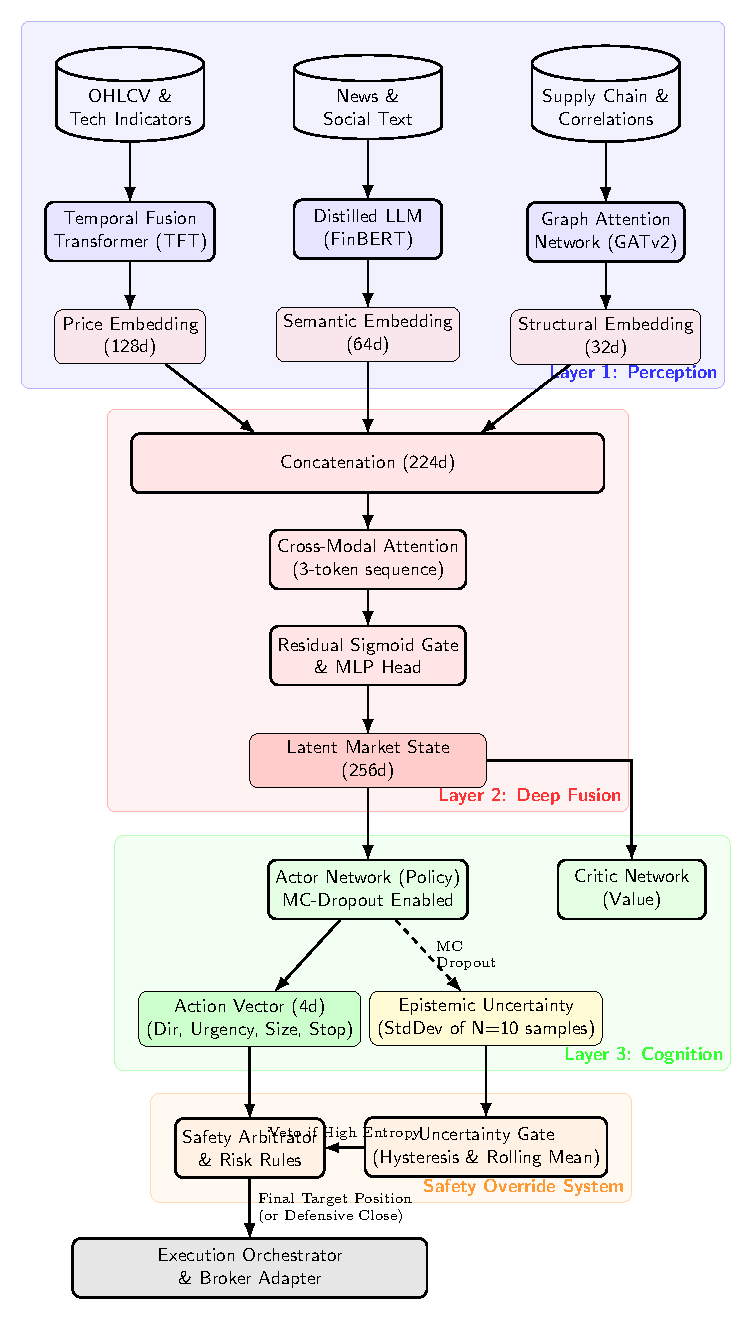
\includegraphics[height=0.82\textheight]{chimera_architecture.pdf}
	\caption{Lumina V3 theoretical topology. The design preserves native modality dimensions
		until the \(224\)-dimensional raw super-vector has been cross-attended and gated.}
	\label{fig:architecture}
\end{figure}

\subsection{Cross-Modal Attention}

The cross-attention block treats the three modalities as three tokens. Each token is read into
a shared attention width \(d_{\mathrm{attn}}=8\times 64=512\), processed by two Transformer
encoder layers, and written back to its native dimension. Let
\[
	q_t = \mathrm{Attn}(p_t,s_t,g_t).
\]
The output is again \(224\)-dimensional:
\[
	h_t=[h_t^{p}\Vert h_t^{s}\Vert h_t^{g}]\in\R^{224}.
\]
The final Nexus computation is
\[
	\gamma_t=\sigma(W_g h_t+b_g),\qquad
	\bar{h}_t = h_t\odot(1+\gamma_t),\qquad
	z_t=H(\bar{h}_t)\in\R^{256},
\]
where \(H\) is the LayerNorm/GELU/dropout MLP head.

\begin{remark}[Why raw concatenation matters]
	The architecture does not first project all modalities to a common width. This is an explicit
	design commitment: price receives 128 coordinates, semantics 64, and graph structure 32
	before the attention block learns how much each modality should matter in context.
\end{remark}

\subsection{State Formation and Attribution}

The fused state is useful only if it remains inspectable. Cross-modal attention weights,
temporal VSN weights, graph edge attention, and semantic attributions form the main
explanation surfaces. They answer different questions: which modality mattered, which
technical variables mattered, which inter-asset edges mattered, and which text tokens mattered.
This interpretability layer is the bridge between V2's explicit indicators and V3's dense
state representation.

\section{Cognition and Control}

\subsection{Action Space}

\begin{definition}[Four-dimensional action]
	The policy action is
	\[
		a_t=(a_t^{(0)},a_t^{(1)},a_t^{(2)},a_t^{(3)})\in[-1,1]^4,
	\]
	with components:
	\[
		\begin{array}{ll}
			a_t^{(0)} & \text{direction: full short to full long},          \\
			a_t^{(1)} & \text{urgency: passive/limit to aggressive/market}, \\
			a_t^{(2)} & \text{sizing: mapped to a risk fraction},           \\
			a_t^{(3)} & \text{stop distance: mapped to ATR multiples}.
		\end{array}
	\]
	The environment decodes sizing through \((a_t^{(2)}+1)/2\) and stop distance through
	\(2.25+1.75a_t^{(3)}\), giving an ATR multiplier in \([0.5,4.0]\).
\end{definition}

The policy supports tanh-squashed diagonal Gaussian actions and a scaled Beta alternative.
The default is the squashed Gaussian:
\[
	\xi_t\sim\mathcal{N}(\mu_\theta(z_t),\sigma_\theta^2),\qquad
	a_t=\tanh(\xi_t),
\]
with the log-probability corrected by the tanh Jacobian.

\subsection{PPO Objective}

The policy is trained with the clipped PPO surrogate objective
\[
	\mathcal{L}^{\mathrm{CLIP}}(\theta)
	=
	\E_t\left[
		\min\left(
		r_t(\theta)\widehat{A}_t,\,
		\clip(r_t(\theta),1-\epsilon,1+\epsilon)\widehat{A}_t
		\right)
		\right],
\]
where
\[
	r_t(\theta)=\frac{\pi_\theta(a_t\mid s_t)}
	{\pi_{\theta_{\mathrm{old}}}(a_t\mid s_t)}.
\]
Advantages are estimated using GAE:
\[
	\delta_t = r_t + \gamma V(s_{t+1})(1-d_t)-V(s_t),
	\qquad
	\widehat{A}_t=\sum_{k\ge 0}(\gamma\lambda)^k\delta_{t+k}.
\]
The update also includes a clipped value loss, entropy bonus, gradient clipping, and KL early
stop.

\subsection{Uncertainty Gate}

For each decision, the policy is sampled \(N=10\) times with dropout active. If
\(a^{(i)}\in[-1,1]^4\) is the \(i\)-th sample, then action-level epistemic uncertainty is
\[
	u_t=\frac{1}{4}\sum_{d=0}^{3}\std_{i=1,\ldots,N}\left(a_d^{(i)}\right).
\]
The gate smooths this with a rolling window of length \(W=10\):
\[
	\bar{u}_t=\frac{1}{W}\sum_{k=t-W+1}^{t}u_k.
\]
It engages when \(\bar{u}_t>\tau_{\mathrm{high}}=0.85\) and releases when
\(\bar{u}_t<\tau_{\mathrm{low}}=0.50\). A 100-step warm-up prevents startup variance from
triggering early vetoes. On veto, the defensive action is the zero vector.

\subsection{Risk-Constrained Action Filtering}

The action \(a_t\) is not treated as an unconditional trade. It is an intent filtered by
deterministic risk rules. The rules can be written abstractly as constraints on exposure,
drawdown, action uncertainty, trade size, stop distance, and loss streaks:
\[
	\mathcal{C}_t(a_t,z_t,E_t,q_t)\le 0.
\]
If the constraint set is violated, the filter maps the proposed action to a safer alternative
such as hold, reduce, or close. This is the V3 analogue of V2's risk analytics layer:
portfolio theory and tail-risk awareness are not after-the-fact reporting tools; they are
embedded in the action boundary itself.

\section{Simulation, Arena, and Feedback}

\subsection{Trading Environment}

A trading environment appends portfolio context to the \(256\)-dimensional market state:
\[
	o_t=[z_t,\ q_t,\ E_t/E_0,\ \mathrm{drawdown}_t,\ t/T]\in\R^{260}.
\]
The step reward used by the base environment is
\[
	R_t
	=
	100\frac{\mathrm{pnl}_t}{E_0}
	-
	\lambda_{\mathrm{risk}}|q_t|\nu_t
	-
	\ind\{\mathrm{arbitrator\ veto}\},
\]
where \(\nu_t\) is recent realized volatility and the default veto penalty is \(1.0\).
Evaluation logs full-episode Sharpe, drawdown, equity, trades, and action traces.

The evaluation language is deliberately continuous with V2. Sharpe, drawdown, transaction
costs, slippage, and stress testing remain the practical yardsticks, while VaR/CVaR and
portfolio-theory concepts such as mean-variance optimization and Black-Litterman
\cite{blacklitterman1992} motivate the safety layer's concern with tail loss, concentration,
and regime fragility. The V3 environment does not solve a Markowitz optimizer inside the
policy; instead, it uses these risk concepts to shape rewards, veto unsafe actions, and
interpret arena outcomes.

\subsection{Risk and Performance Functionals}

For portfolio return \(R_p\), risk-free return \(R_f\), and portfolio volatility
\(\sigma_p\), the Sharpe ratio is
\[
	\mathrm{SR}=\frac{\E[R_p]-R_f}{\sigma_p}.
\]
Drawdown is computed from the equity curve \(E_t\) as
\[
	\mathrm{DD}_t = 1-\frac{E_t}{\max_{s\le t}E_s},
	\qquad
	\mathrm{MDD}=\max_t \mathrm{DD}_t.
\]
Tail risk is represented by Value at Risk and Conditional Value at Risk:
\[
	\mathrm{VaR}_{\alpha}(L)=\inf\{\ell:\Pr(L\le \ell)\ge \alpha\},
	\qquad
	\mathrm{CVaR}_{\alpha}(L)=\E[L\mid L\ge \mathrm{VaR}_{\alpha}(L)].
\]
These quantities supply the language for comparing policies under stress even when the
optimization target is a reinforcement-learning reward rather than a closed-form portfolio
objective.

\subsection{Adversarial Generators}

The domain-randomization stage can warp episodes with six perturbations:
flash crash, sustained crash, volatility spike, correlation break, semantic panic, and silent
drift. The default training mix is \(70\%\) clean episodes and \(30\%\) adversarial episodes.
Synthetic sanity episodes support geometric Brownian motion and Merton jump diffusion.
This preserves the V2 backtesting discipline of walk-forward validation, transaction-cost
awareness, and Monte Carlo scenario analysis \cite{delprado2018}; the difference is that V3
uses the scenarios to expose policy behavior and generate counterfactual feedback, not only
to score a fixed strategy.

\begin{figure}[htbp]
	\centering
	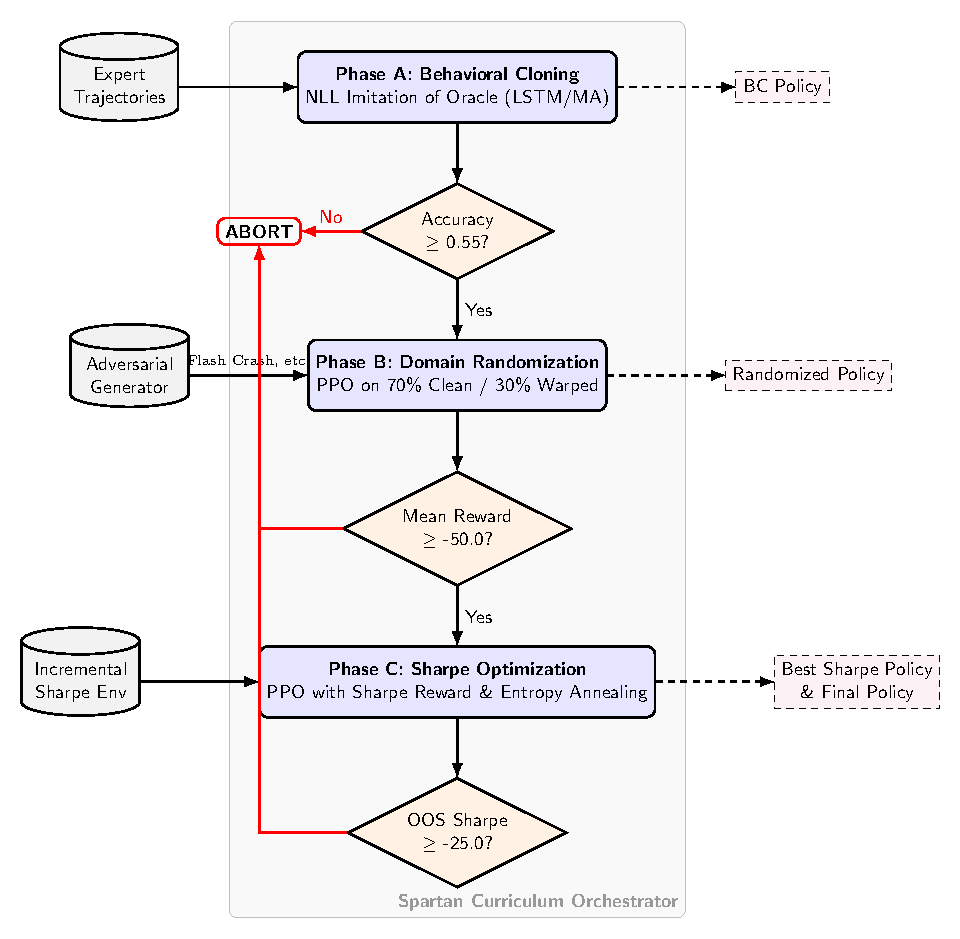
\includegraphics[width=0.82\textwidth]{spartan_curriculum.pdf}
	\caption{Spartan curriculum structure. Behavioral cloning establishes an initial policy,
		domain randomization stress-tests it against warped market trajectories, and Sharpe-oriented
		optimization refines the policy under explicit acceptance gates.}
	\label{fig:spartan-curriculum}
\end{figure}

\subsection{Spartan Arena}

The Spartan Arena runs \(N\) trajectories step-locked over a shared scenario. For each step,
the divergence analyzer computes the pairwise action spread and subsequent Sharpe spread over
a horizon \(K=30\):
\[
	d_k=\max_{i,j}\|a_{i,k}-a_{j,k}\|_2,\qquad
	\Delta S_k = \max_i S_{i,k:k+K}-\min_i S_{i,k:k+K}.
\]
A divergence is pivotal when
\[
	d_k\ge 0.15,\qquad \Delta S_k\ge 0.15.
\]
Each pivotal divergence becomes a counterfactual pair: same state, good action, bad action,
and two outcome Sharpes.

\begin{figure}[htbp]
	\centering
	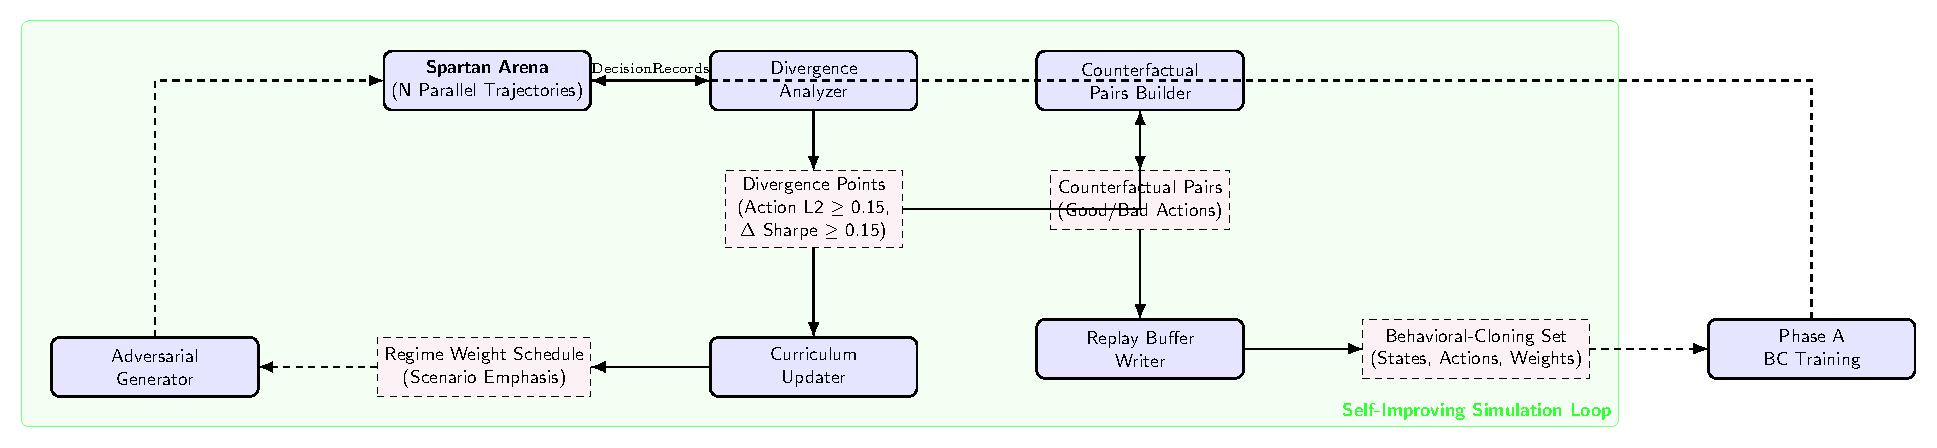
\includegraphics[width=\textwidth]{arena_feedback_loop.pdf}
	\caption{Spartan Arena feedback loop. Shared scenarios expose action divergences, convert them
		into good-action/bad-action pairs, and evaluate whether behavioral cloning reduces repeated
		decision errors.}
	\label{fig:arena-loop}
\end{figure}

\section{Factor and Regime Structure}

The V2 draft includes classical factor models because prediction is not the only problem:
the agent must understand whether returns are driven by broad market exposure, size, value,
profitability, investment, momentum, or idiosyncratic structure. The CAPM baseline is
\[
	\E[R_i]=R_f+\beta_i(\E[R_m]-R_f),
	\qquad
	\beta_i=\frac{\mathrm{Cov}(R_i,R_m)}{\mathrm{Var}(R_m)}.
\]
Fama-French and Carhart models enrich this with persistent risk premia:
\[
	R_i-R_f
	=
	\alpha_i+\beta_i^{MKT}MKT+\beta_i^{SMB}SMB+\beta_i^{HML}HML
	+\beta_i^{MOM}MOM+\epsilon_i.
\]
V3 does not need to hard-code these factors into the action rule, but factor exposure remains
the right language for diagnosing whether a learned policy is discovering alpha or merely
levering a known beta.

Regime structure is the other half of this diagnosis. In V2, regimes are described through
bull, bear, sideways, high-volatility, and low-volatility states, with tools such as hidden
Markov models and GARCH-family volatility. In V3, regime information can appear as a temporal
head, an adversarial scenario label, a graph-state change, or a safety trigger. The theoretical
point is the same: market efficiency and exploitable structure are time-varying, so a policy
must be evaluated conditionally rather than only by aggregate return.

\section{Validation Methodology}

The paper should be read as a theoretical review, but the theory still imposes strict
validation rules. The central constraint is chronological causality: training statistics,
normalizers, feature windows, labels, and risk estimates must be formed without future
information. Walk-forward evaluation expresses this constraint:
\[
	[\mathrm{Train}_1][\mathrm{Val}_1],\quad
	[\mathrm{Train}_2][\mathrm{Val}_2],\quad \ldots
\]
Purged cross-validation \cite{delprado2018} further removes samples whose label horizons
overlap the validation interval and inserts an embargo to reduce leakage.

Transaction costs also belong to the theoretical model, not just to deployment. If
\(C_{\mathrm{comm}}\), \(C_{\mathrm{spread}}\), \(C_{\mathrm{impact}}\), and
\(C_{\mathrm{slippage}}\) denote commission, spread, market impact, and slippage, then
\[
	TC=C_{\mathrm{comm}}+C_{\mathrm{spread}}+C_{\mathrm{impact}}+C_{\mathrm{slippage}}.
\]
A policy that wins before costs but loses after costs has not solved the trading problem.
Monte Carlo perturbations, bootstrap resampling, geometric Brownian motion, Merton jump
diffusion \cite{merton1976}, and adversarial scenarios are therefore used to ask whether the
state-action rule is stable under market variation rather than merely fitted to one history.

\subsection{Simulation Sequence Evolution}

Across nine recorded article simulations, the experimental sequence moved from small-universe
diagnostic runs to broader-universe partial-learning runs. The first seven simulations used
\(291{,}457\) daily OHLCV rows over 33 tickers; the final two expanded the universe to
\(523{,}345\) and \(531{,}073\) rows over 52 and 54 tickers, respectively. All nine
simulations share an important data boundary: the text and supply-chain modalities are absent,
so the evidence primarily tests the price encoder, correlation graph, fusion layer, policy,
and feedback loop.

\begin{table}[htbp]
	\centering
	\scriptsize
	\caption{Chronological evolution across the nine recorded article simulations. Directional
		accuracy is reported after the hard-example pass and compared with the naive sign baseline.
		\(\Delta S_{VT}\) is the mean post-feedback minus baseline Sharpe change across the validation
		and test scenarios.}
	\label{tab:simulation-evolution}
	\begin{tabular}{clcccccc}
		\toprule
		Cycle & Status & Rows/tickers & Val. MSE & Test dir. & Naive dir. & BC acc. & \(\Delta S_{VT}\) \\
		\midrule
		1 & Inconclusive & 291k / 33 & \(0.005187\to0.010272\) & 0.509 & 0.552 & 0.027 & -0.008 \\
		2 & Inconclusive & 291k / 33 & \(0.005305\to0.011877\) & 0.487 & 0.552 & 0.161 &  0.009 \\
		3 & Inconclusive & 291k / 33 & \(0.004806\to0.004728\) & 0.583 & 0.552 & 0.484 & -0.005 \\
		4 & Inconclusive & 291k / 33 & \(0.004852\to0.006020\) & 0.560 & 0.552 & 0.140 &  0.041 \\
		5 & Inconclusive & 291k / 33 & \(0.005116\to0.004944\) & 0.536 & 0.552 & 0.106 & -2.230 \\
		6 & Partial      & 291k / 33 & \(0.005053\to0.005053\) & 0.559 & 0.552 & 0.658 &  0.013 \\
		7 & Learned      & 291k / 33 & \(0.004728\to0.004689\) & 0.583 & 0.552 & 0.742 &  0.027 \\
		8 & Partial      & 523k / 52 & \(0.005219\to0.005189\) & 0.569 & 0.539 & 0.560 & -0.001 \\
		9 & Partial      & 531k / 54 & \(0.005570\to0.005570\) & 0.567 & 0.540 & 0.549 &  0.000 \\
		\bottomrule
	\end{tabular}
\end{table}

The sequence shows three lessons. First, the hard-example pass is not automatically
beneficial: validation MSE improved in four cycles, was effectively unchanged in two, and
worsened in three. Second, directional accuracy became more reliable than raw MSE as the
control-relevant signal: six of nine cycles finished above the naive directional baseline,
with the strongest edge around \(0.583\) versus \(0.552\) in the 33-ticker setting and around
\(0.568\) versus \(0.540\) after expanding the universe. Third, counterfactual feedback is
powerful but not monotone. The sequence produced 345 counterfactual pairs and 850 feedback
samples, while behavioral-cloning sign accuracy ranged from \(0.027\) to \(0.742\). The
fifth cycle demonstrates the failure mode: feedback can over-correct and damage stress
Sharpe. The learned cycle shows the constructive case: validation MSE improves, test
directional accuracy exceeds the naive baseline, behavioral cloning reaches \(0.742\), and
post-feedback Sharpe improves in two of the three validation/test scenarios. The broader
universe cycles preserve a positive directional edge but reduce the feedback gain to roughly
neutral, indicating that the enlarged state space needs stronger calibration rather than
larger claims.

The 54-ticker expanded-universe simulation gives a more detailed view of that last point.
Figure \ref{fig:nexus-optimization-dynamics} separates the two optimization passes. The
initial pass rapidly compresses training loss and then enters a shallow improvement regime;
the hard-example pass is short, validation-monitored, and ultimately restores the best
validation level rather than accepting a later noisy epoch. This is useful evidence for the
paper's main safety claim: the hard-example mechanism acts as a selective correction layer,
not as an unconditional second training phase.

\begin{figure}[htbp]
	\centering
	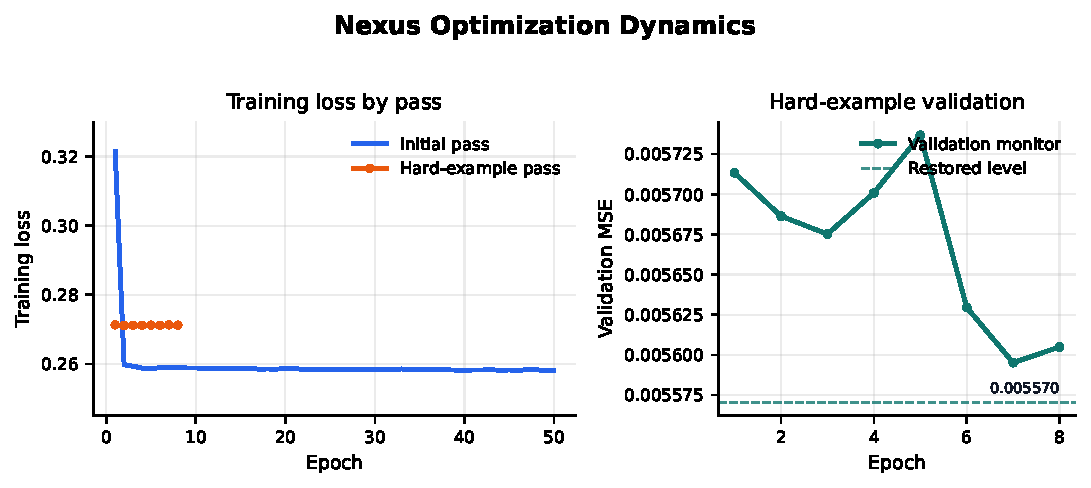
\includegraphics[width=0.94\textwidth]{nexus_optimization_dynamics.pdf}
	\caption{Nexus optimization dynamics for the expanded-universe simulation. The initial
		pass performs most of the loss compression, while the hard-example pass is governed by
		validation monitoring and early restoration.}
	\label{fig:nexus-optimization-dynamics}
\end{figure}

The same simulation also shows why the article treats directional accuracy as a
control-relevant diagnostic rather than using MSE alone. Figure
\ref{fig:nexus-directional-edge} compares the model's directional accuracy against a naive
sign baseline on each chronological split. The edge remains positive on train, validation,
and test slices, with the strongest separation on validation and a smaller but still positive
test margin.

\begin{figure}[htbp]
	\centering
	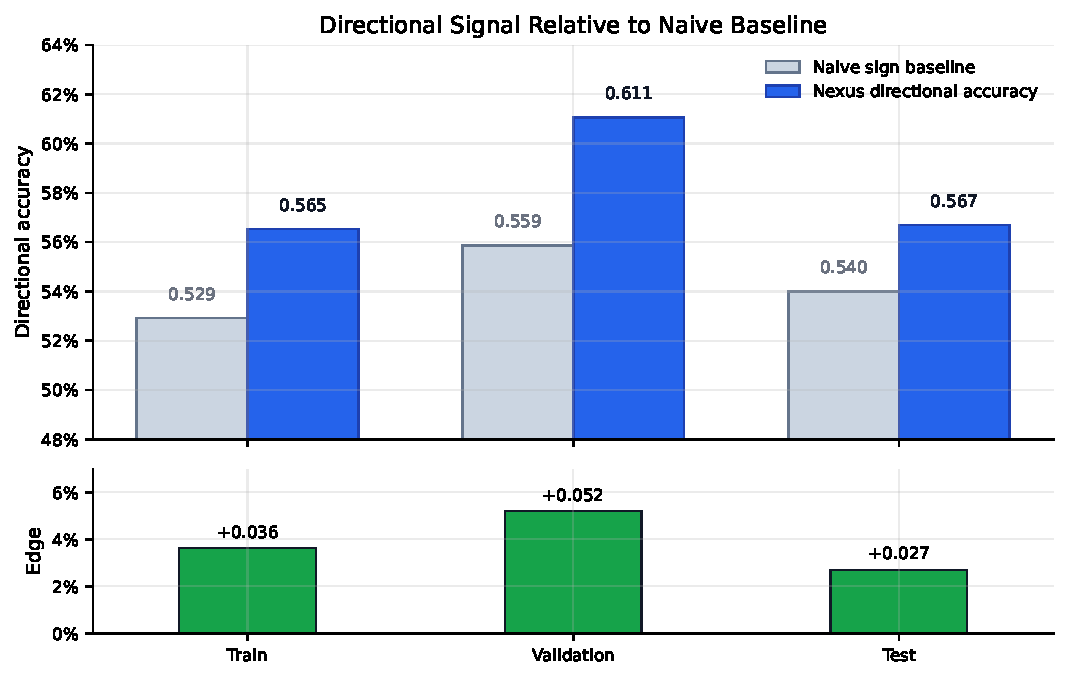
\includegraphics[width=0.9\textwidth]{nexus_directional_edge.pdf}
	\caption{Directional signal relative to the naive sign baseline. The model keeps a
		positive directional edge across train, validation, and test slices even when the
		validation MSE is unchanged by the hard-example pass.}
	\label{fig:nexus-directional-edge}
\end{figure}

Figure \ref{fig:expanded-split-scale} records the chronological sample scale behind those
metrics. The train segment dominates the supervised signal, while the validation and test
segments remain large enough to expose whether the directional edge survives outside the
fitting interval.

\begin{figure}[htbp]
	\centering
	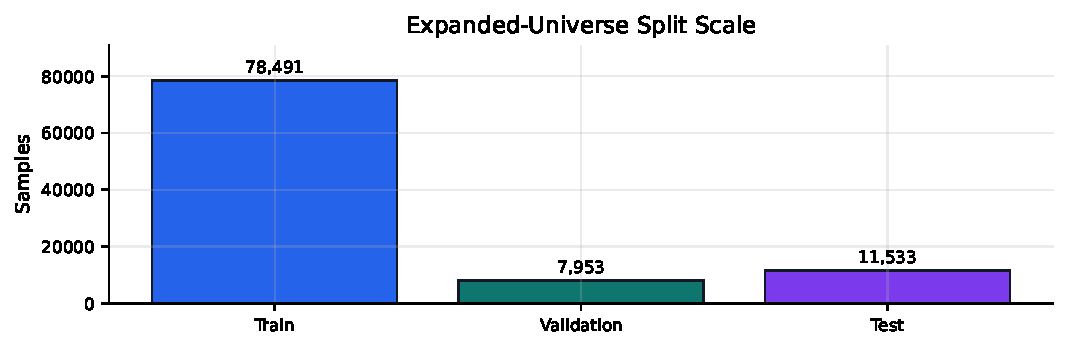
\includegraphics[width=0.78\textwidth]{nexus_split_scale.pdf}
	\caption{Sample scale of the expanded-universe split. The asymmetric split emphasizes
		large historical training coverage while preserving separate validation and test
		windows for chronological assessment.}
	\label{fig:expanded-split-scale}
\end{figure}

The arena results in Figure \ref{fig:arena-feedback-scenario-effects} explain the
partial-learning classification. Feedback increases total return in all displayed scenarios
and moves the policy away from the counterfactual action references, but Sharpe changes are
near neutral and drawdowns generally become deeper. The behavioral interpretation is
therefore conservative: the feedback loop changes action geometry and can improve raw return,
but its risk-adjusted effect requires stronger calibration before it should be treated as a
stable control improvement.

\begin{figure}[htbp]
	\centering
	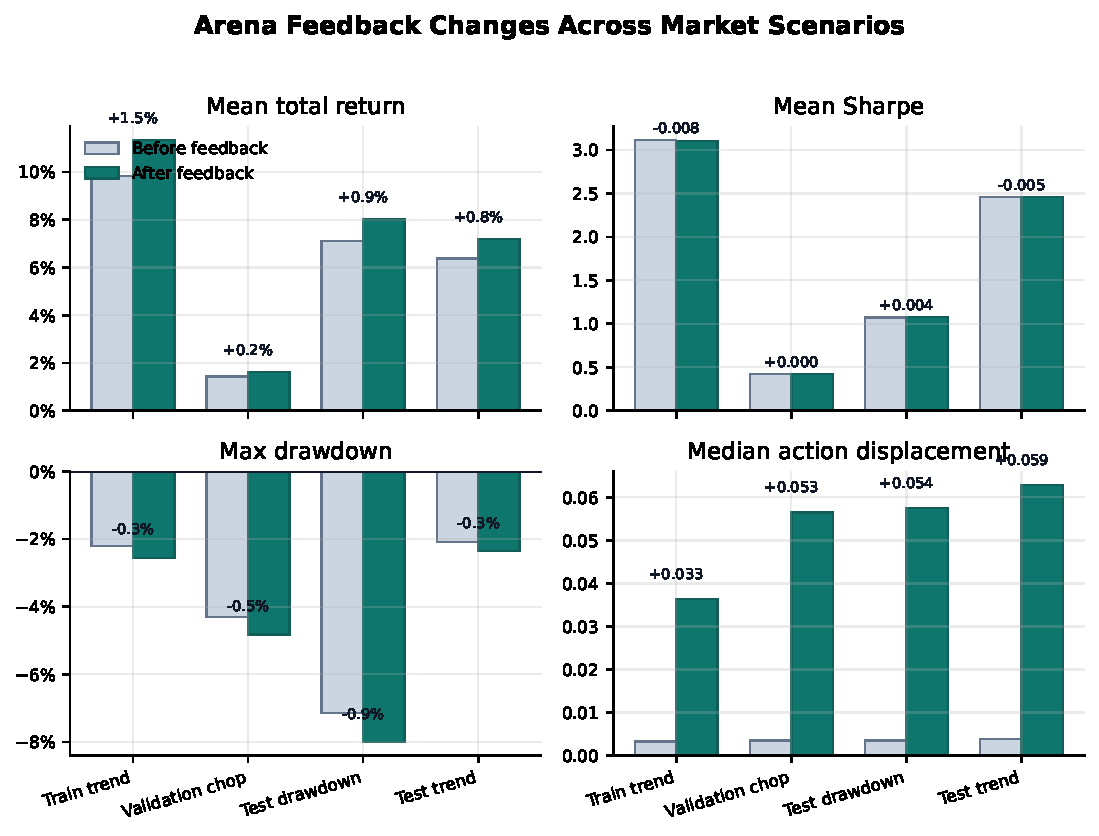
\includegraphics[width=0.96\textwidth]{arena_feedback_scenario_effects.pdf}
	\caption{Arena feedback effects across trend, chop, and drawdown scenarios. The feedback
		layer increases return and action displacement, while Sharpe remains approximately
		neutral and drawdown risk increases.}
	\label{fig:arena-feedback-scenario-effects}
\end{figure}

\subsection{Crisis Drill Response}

The arena scenarios are complemented by two synthetic tail-regime drills: a crypto winter
trajectory and a Lehman-style collapse. These drills are not presented as production guarantees.
Their purpose is narrower and theoretical: they test whether the composition of perception,
uncertainty estimation, policy control, and safety arbitration behaves differently when the
market trajectory leaves ordinary calibration territory.

\begin{table}[htbp]
	\centering
	\small
	\caption{Crisis-drill response under severe tail regimes. Asset move is measured from
		the first to the last scenario step; maximum drawdown is measured from the portfolio
		equity curve.}
	\label{tab:crisis-drills}
	\begin{tabular}{lrrrrr}
		\toprule
		Scenario & Asset move & Portfolio move & Max. drawdown & Safety vetoes & Max. uncertainty \\
		\midrule
		Crypto winter  & \(-59.7\%\) & \(-2.7\%\) & \(-5.1\%\) &  7 & 0.939 \\
		Lehman moment  & \(-97.9\%\) & \(+0.3\%\) & \(-0.8\%\) & 18 & 0.979 \\
		\bottomrule
	\end{tabular}
\end{table}

Figure \ref{fig:crisis-drill-tail-response} shows that the two drills stress different
failure modes. In the crypto winter case, the asset first rallies and then collapses; the
policy repeatedly re-enters with small exposure, uncertainty rises above the veto threshold
seven times, and portfolio loss is contained but not eliminated. This is a whipsaw-resilience
test: the model must decide whether a violent decline is temporary mean reversion or a regime
break. In the Lehman-style collapse, the asset loses almost all of its value after the shock;
uncertainty jumps above the veto threshold, exposure is reduced to zero after the first
crisis veto, and the portfolio avoids the tail of the collapse. This is a kill-switch test:
the correct behavior is not clever re-optimization but refusal to keep trading into an
unmodelled discontinuity.

\begin{figure}[htbp]
	\centering
	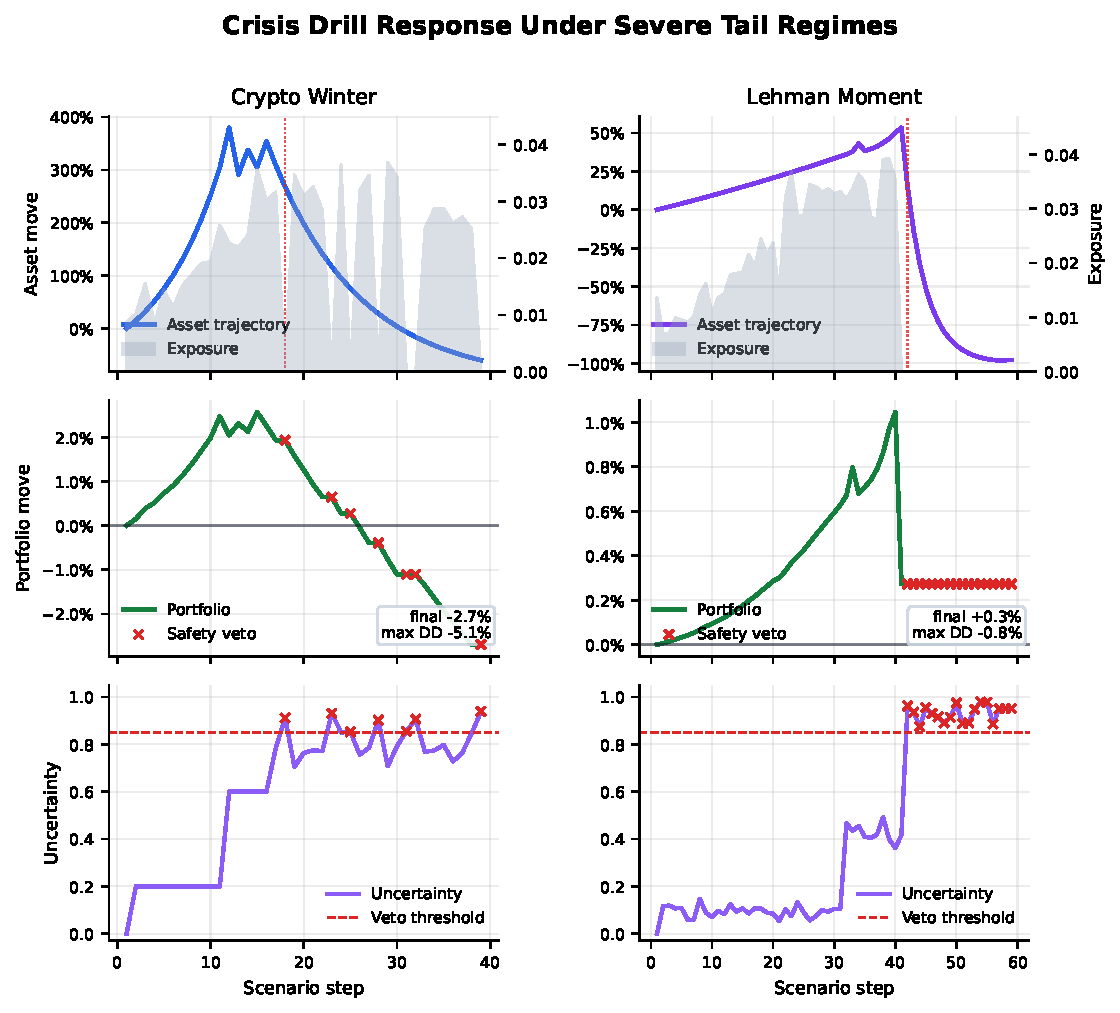
\includegraphics[width=0.98\textwidth]{crisis_drill_tail_response.pdf}
	\caption{Crisis-drill behavior under crypto winter and Lehman-style collapse regimes. The
		upper panels compare normalized asset moves with exposure, the middle panels show
		portfolio response and safety vetoes, and the lower panels show uncertainty against the
		veto threshold.}
	\label{fig:crisis-drill-tail-response}
\end{figure}

The difference between the two responses is important. A severe but continuous crypto decline
still leaves room for small, repeatedly reassessed positions; a discontinuous banking-crisis
collapse should push the safety layer toward abstention. The stress evidence therefore
supports a central design principle of Lumina V3: the controller is not only a return
maximizer, but a gated decision process whose safest action under epistemic stress may be no
action.

\subsection{Latency and Operational Feasibility}

Operational integrity is measured by the latency of the end-to-end inference cycle, or
``Reflex Arc.'' Figure \ref{fig:latency-profile} details the latency percentiles measured over
10,000 cycles.

\begin{figure}[htbp]
	\centering
	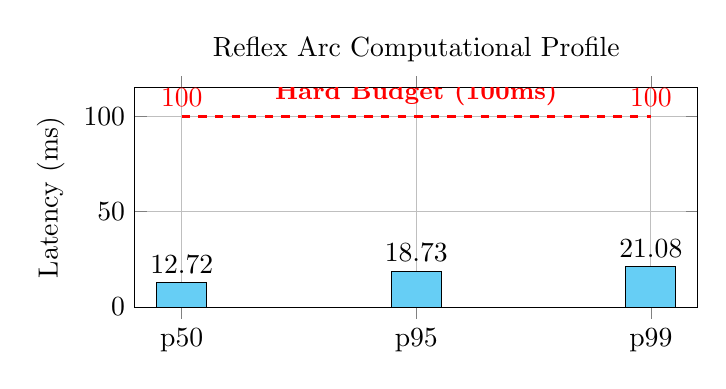
\begin{tikzpicture}
		\begin{axis}[
				width=0.72\textwidth,
				height=0.36\textwidth,
				ybar,
				bar width=18pt,
				symbolic x coords={p50, p95, p99},
				xtick=data,
				ylabel={Latency (ms)},
				title={Reflex Arc Computational Profile},
				ymin=0,
				ymax=115,
				nodes near coords,
				grid=major,
			]
			\addplot[fill=cyan!60, draw=black] coordinates {
					(p50, 12.72)
					(p95, 18.73)
					(p99, 21.08)
				};
			\addplot[red, sharp plot, dashed, thick, update limits=false]
			coordinates {(p50, 100) (p99, 100)}
			node[above, pos=0.5, font=\small\bfseries] {Hard Budget (100ms)};
		\end{axis}
	\end{tikzpicture}
	\caption{Reflex arc latency profile. Computational overhead remains significantly below the
		required threshold for high-frequency decision making, validating the use of the distilled
		perception stack.}
	\label{fig:latency-profile}
\end{figure}

\section{Abstract System Composition}

At the highest level, Lumina V3 is a composition of maps:
\[
	\mathcal{D}
	\xrightarrow{\ \Phi\ }
	(W_t,N_t,G_t)
	\xrightarrow{\ E_{\mathrm{price}},E_{\mathrm{sem}},E_{\mathrm{graph}}\ }
	(p_t,s_t,g_t)
	\xrightarrow{\ F_{\mathrm{nexus}}\ }
	z_t
	\xrightarrow{\ \pi_\theta\ }
	a_t
	\xrightarrow{\ \mathcal{A}\ }
	\tilde{a}_t.
\]
Here \(\mathcal{D}\) is the market-data process, \(\Phi\) is feature construction,
\(F_{\mathrm{nexus}}\) is multimodal fusion, \(\pi_\theta\) is the stochastic policy, and
\(\mathcal{A}\) is the risk filter that maps an intended action to an executable action or to
hold/close. This is the clean theoretical shape of the project. Engineering choices should
preserve this composition rather than define the paper's argument.

\section{Limitations}

Four limitations follow from the theoretical framing.

\begin{enumerate}
	\item The V3 architecture is richer than any single data source. If semantic events,
	      relation graphs, or high-frequency features are absent, the corresponding theoretical
	      modality cannot be validated.

	\item The paper does not claim empirical Lumina V2-vs-V3 parity because the historical V2
	      baseline is not available for reproduction. V2 is used here as lineage, theoretical
	      context, and architectural contrast rather than as a reproduced benchmark.

	\item Reinforcement learning can overfit scenario design. A persuasive evaluation must cover
	      temporal splits, costs, stress regimes, uncertainty, factor exposure, and tail risk.

	\item The theory is a research framework, not an investment guarantee. A mathematically
	      coherent policy can still fail under distribution shift, liquidity constraints, data
	      errors, or changing market microstructure.
\end{enumerate}

\section{Conclusion}

Lumina V3 is best understood as a theoretical reorganization of Lumina V2. V2 supplied the
classical quantitative-finance foundation: adaptive market efficiency, stochastic price
processes, technical indicators, sequence models, factor analysis, risk metrics, sentiment,
and backtesting discipline. V3 keeps that foundation but moves the decision boundary from a
linear research pipeline into a multimodal latent state and a risk-constrained policy. The
main advance is therefore not the abandonment of classical quantitative finance; it is the
relocation of those concepts into a fused, auditable, safety-aware control loop.

\appendix

\section{Mathematical Summary}

\begin{longtable}{p{0.30\textwidth}p{0.58\textwidth}}
	\caption{Core theoretical objects retained from V2 and reorganized in V3.}
	\label{tab:math-summary}                                                                          \\
	\toprule
	Object                                   & Role in the Lumina framework                           \\
	\midrule
	\endfirsthead
	\toprule
	Object                                   & Role in the Lumina framework                           \\
	\midrule
	\endhead
	Log return \(r_t=\log(P_t/P_{t-1})\)     & Canonical stationary target and input
	transformation for price movement.                                                                \\
	Technical indicators                     & Interpretable V2 feature family used as V3 temporal
	inputs and attribution anchors.                                                                   \\
	Volatility estimators                    & Scale variables for normalization, reward shaping,
	stop distance, stress testing, and risk filters.                                                  \\
	Sentiment decay \(e^{-\lambda\Delta t}\) & V2 scalar news model generalized by
	V3 semantic embeddings.                                                                           \\
	Relation graph \(G_t\)                   & Encodes cross-asset correlation, economic links, and
	factor co-movement for structural embeddings.                                                     \\
	Fusion state \(z_t\in\R^{256}\)          & Shared latent market state on which the policy acts.   \\
	Action \(a_t\in[-1,1]^4\)                & Continuous decision vocabulary for direction,
	urgency, sizing, and stop distance.                                                               \\
	Uncertainty \(u_t\)                      & Epistemic dispersion estimate used to gate unsafe or
	unstable actions.                                                                                 \\
	Risk metrics                             & Sharpe, drawdown, VaR/CVaR, costs, and factor exposure
	define evaluation beyond raw return.                                                              \\
	Walk-forward validation                  & Chronological evaluation discipline inherited from V2
	and required for any V3 empirical claim.                                                          \\
	\bottomrule
\end{longtable}

\section{References}

\begin{thebibliography}{99}

	\bibitem{aitchison1986}
	Aitchison, J. (1986).
	\newblock \emph{The Statistical Analysis of Compositional Data}.
	\newblock Chapman and Hall.

	\bibitem{blacklitterman1992}
	Black, F. and Litterman, R. (1992).
	\newblock Global portfolio optimization.
	\newblock \emph{Financial Analysts Journal}, 48(5):28--43.

	\bibitem{bollinger1980}
	Bollinger, J. (1980).
	\newblock \emph{Bollinger on Bollinger Bands}.
	\newblock McGraw-Hill.

	\bibitem{bollerslev1986}
	Bollerslev, T. (1986).
	\newblock Generalized autoregressive conditional heteroskedasticity.
	\newblock \emph{Journal of Econometrics}, 31(3):307--327.

	\bibitem{brody2022}
	Brody, S., Alon, U., and Yahav, E. (2022).
	\newblock How attentive are graph attention networks?
	\newblock \emph{International Conference on Learning Representations}.

	\bibitem{carhart1997}
	Carhart, M. M. (1997).
	\newblock On persistence in mutual fund performance.
	\newblock \emph{The Journal of Finance}, 52(1):57--82.

	\bibitem{chou2017}
	Chou, P.-W., Maturana, D., and Scherer, S. (2017).
	\newblock Improving stochastic policy gradients in continuous control with deep reinforcement
	learning using the beta distribution.
	\newblock \emph{International Conference on Machine Learning}.

	\bibitem{delprado2018}
	de Prado, M. L. (2018).
	\newblock \emph{Advances in Financial Machine Learning}.
	\newblock Wiley.

	\bibitem{engstrom2020}
	Engstrom, L., Ilyas, A., Santurkar, S., Tsipras, D., Janoos, F., Rudolph, L., and Madry, A. (2020).
	\newblock Implementation matters in deep RL: A case study on PPO and TRPO.
	\newblock \emph{International Conference on Learning Representations}.

	\bibitem{fama1993}
	Fama, E. F. and French, K. R. (1993).
	\newblock Common risk factors in the returns on stocks and bonds.
	\newblock \emph{Journal of Financial Economics}, 33(1):3--56.

	\bibitem{fama2015}
	Fama, E. F. and French, K. R. (2015).
	\newblock A five-factor asset pricing model.
	\newblock \emph{Journal of Financial Economics}, 116(1):1--22.

	\bibitem{gal2016}
	Gal, Y. and Ghahramani, Z. (2016).
	\newblock Dropout as a Bayesian approximation: Representing model uncertainty in deep learning.
	\newblock \emph{International Conference on Machine Learning}.

	\bibitem{haarnoja2018}
	Haarnoja, T., Zhou, A., Abbeel, P., and Levine, S. (2018).
	\newblock Soft actor-critic: Off-policy maximum entropy deep reinforcement learning with a
	stochastic actor.
	\newblock \emph{International Conference on Machine Learning}.

	\bibitem{hochreiter1997}
	Hochreiter, S. and Schmidhuber, J. (1997).
	\newblock Long short-term memory.
	\newblock \emph{Neural Computation}, 9(8):1735--1780.

	\bibitem{lim2021}
	Lim, B., Arik, S. O., Loeff, N., and Pfister, T. (2021).
	\newblock Temporal Fusion Transformers for interpretable multi-horizon time series forecasting.
	\newblock \emph{International Journal of Forecasting}, 37(4):1748--1764.

	\bibitem{lo2004}
	Lo, A. W. (2004).
	\newblock The adaptive markets hypothesis.
	\newblock \emph{The Journal of Portfolio Management}, 30(5):15--29.

	\bibitem{markowitz1952}
	Markowitz, H. (1952).
	\newblock Portfolio selection.
	\newblock \emph{The Journal of Finance}, 7(1):77--91.

	\bibitem{merton1976}
	Merton, R. C. (1976).
	\newblock Option pricing when underlying stock returns are discontinuous.
	\newblock \emph{Journal of Financial Economics}, 3(1--2):125--144.

	\bibitem{moody2001}
	Moody, J. and Saffell, M. (2001).
	\newblock Learning to trade via direct reinforcement.
	\newblock \emph{IEEE Transactions on Neural Networks}, 12(4):875--889.

	\bibitem{schulman2016}
	Schulman, J., Moritz, P., Levine, S., Jordan, M., and Abbeel, P. (2016).
	\newblock High-dimensional continuous control using generalized advantage estimation.
	\newblock \emph{International Conference on Learning Representations}.

	\bibitem{schulman2017}
	Schulman, J., Wolski, F., Dhariwal, P., Radford, A., and Klimov, O. (2017).
	\newblock Proximal policy optimization algorithms.
	\newblock arXiv:1707.06347.

	\bibitem{sharpe1966}
	Sharpe, W. F. (1966).
	\newblock Mutual fund performance.
	\newblock \emph{The Journal of Business}, 39(1):119--138.

	\bibitem{tsai2019}
	Tsai, Y.-H. H., Bai, S., Liang, P. P., Kolter, J. Z., Morency, L.-P., and Salakhutdinov, R. (2019).
	\newblock Multimodal Transformer for unaligned multimodal language sequences.
	\newblock \emph{ACL}.

	\bibitem{vaswani2017}
	Vaswani, A., Shazeer, N., Parmar, N., Uszkoreit, J., Jones, L., Gomez, A. N., Kaiser, L.,
	and Polosukhin, I. (2017).
	\newblock Attention is all you need.
	\newblock \emph{NeurIPS}.

	\bibitem{wilder1978}
	Wilder, J. W. (1978).
	\newblock \emph{New Concepts in Technical Trading Systems}.
	\newblock Trend Research.

\end{thebibliography}

\end{document}
